\section{Biography}
\begin{centering}
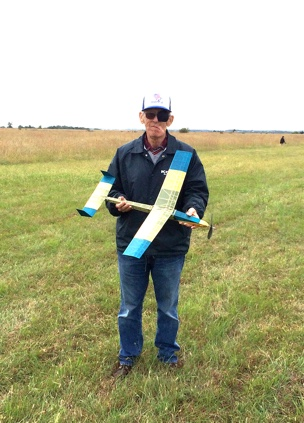
\includegraphics[width=0.45\textwidth]{../assets/images/RoieBlack.jpg}
\end{centering}

In the Summer of 1955 I was delivering the evening newspaper in Falls Church,
Virginia, when I rounded the corner of an apartment building and saw a man
release the propeller on a rubber-powered model airplane. The plane circled in
front of this man's home for several minutes, and magically landed where it had
started. The airplane was a Henderson Gadfly, published in Model Airplane News
that year.  I was fascinated by that sight, and decided to figure out how the
airplane managed to do that. I talked the man into giving me the plans he used
to build the model, traced from the magazine. I still has those plans to this
day!) Soon, a couple of my friends and I decided to start building model
airplanes of our own.  We all took a bus to downtown Washington, D.C (kids
could do that back then), and joined the Academy of Model Aeronautics. We also
joined the {\it Fairfax Model Associates} and began competing in a variety of events,
mostly control line and gas free flight. At one meeting, Bill Bigge, an
internationally known indoor model builder, was the guest speaker. I got my
first look at a new form of model airplane. The indoor models Bill brought to
the meeting were fascinating, and cheap enough even a kid with a limited
allowance could build one.  Bill became my mentor, and  I managed to build an
ornithopter and helicopter and set two national records! After almost getting a
PhD in Aerospace Engineering from Virginia Tech, I spent 20 years as an
officer in the USAF, then got a second Master's degree in Computer Science and
spent another 17 years teaching college-level Computer Science. I finally
retired for good in 2018, and moved with my wife to Kansas City, where I joined
the {\it  Heart of America Free Flight Association}, and again began flying model
airplanes, this time focusing on rubber and electric powered outdoor free
flight, and indoor events.When not building model airplanes, I am active in
Amateur Radio and am currently authoring a book on Computer Architecture.
